
Существуют два подхода к проблеме построения накопительного кольца для измерения ЭДМ дейтрона: 
\begin{enumerate*}[\itshape a\upshape)]
	\item структура с ``замороженным'' спином (FS), и 
	\item структура с ``квази-замороженным'' спином (QFS).
\end{enumerate*}

В следующих разделах мы рассмотрим возможные варианты колец обоих типов.

\section{Структура с ``замороженным'' спином} \label{chpt2:lattice:FS_BNL}
В структуре FS-типа, горизонтальная проекция вектора спина частицы пучка \emph{непрерывно} сонаправлена с вектором её импульса. Для реализации условия непрерывности, в такой структуре используются цилиндрические спин-ротаторы, создающие одновременно и электростатическое, и магнитное поля. На Рисунке~\ref{fig:BNL_lattice} представлен вариант кольца FS-типа.~\cite{Senichev:Lattices} Данное кольцо имеет длину 145.85~м, и рассчитано на инжекцию пучка дейтронов на энергии 270 МэВ. В структуре предусмотрено использование ВЧ-резонатора для подавления линейного эффекта декогеренции спина путём усреднения энергии вокруг значения равновесной энергии частицы. Продольное напряжение резонатора $V = 100$ кВ, частота поля $f_{RF} = 5\cdot f_{rev}$, где частота оборота пучка $f_{rev} = 1.00$ МГц. Остающиеся нелинейные эффекты декогеренции подавляются с помощью трёх\footnote{Некоторые авторы используют
два семейства~\cite{Eremey:Thesis} в этой структуре.} семейств секступолей.

\begin{figure}[h!]
	\centering
	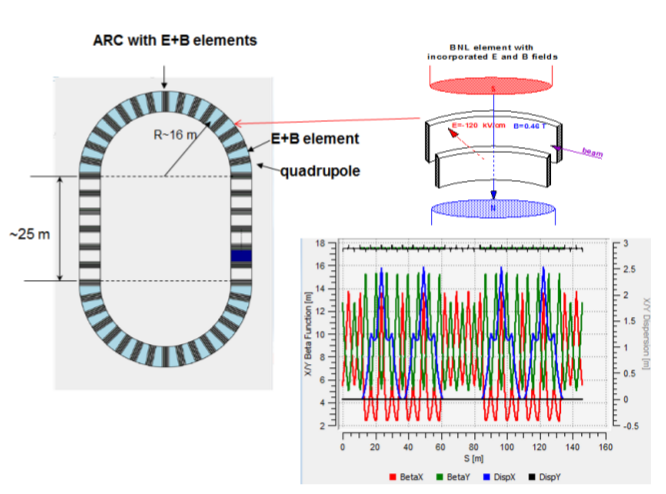
\includegraphics[width=\linewidth]{images/chapter2/BNL_lattice}
	\caption{Вариант кольца, построенного по принципу ``замороженного'' спина. В арках использованы цилиндрические электро-магнитные элементы (Рисунок взят из~\cite{Senichev:Lattices})\label{fig:BNL_lattice}}
\end{figure}

Основная цель FS-концепции кольца --- максимизация ЭДМ сигнала. Однако, следует обратить внимание на то, что строгое выполнение условия замороженности спина возможно только для референсной частицы. Это связано с тем, что, как следует из уравнения~\eqref{eq:TBMT_MDM}, для заданных E-, B-полей, существует уникальное значение Лоренц-фактора $\gamma$, при котором $\W_y^{MDM} = 0$. Таким образом, даже в FS-структуре, спин-векторы большинства частиц ``заморожены'' лишь приблизительно.

\section{Структура с ``квази-замороженным'' спином} \label{chpt2:concept:QFS}
В QFS-концепции кольца отказываются от непрерывного выполнения условия сонаправленности векторов поляризации и импульса пучка, требуя лишь равенства нулю \emph{совокупного за оборот} угла поворота вектора поляризации относительно импульса в электростатических ($\Phi_s^E$) и магнитных ($\Phi_s^B$) элементах (углы отсчитываются в системе центра масс):~\cite{Senichev:Lattices}
\begin{equation*}
	\sum_i \Phi_{s,i}^E = -\sum_j \Phi_{s,j}^B.
\end{equation*}

Как следует из определения спин-тюна (см. раздел~\ref{sec:TBMT_introduction}), угол поворота спин-вектора частицы относительно её импульса в электромагнитном поле $\Phi_s = \nu_s \cdot \Phi$, где $\Phi$ угол поворота импульса, а $\nu_s$ спин-тюн.

Угловая скорость поворота вектора импульса частицы в магнитном поле $\vec B$ есть 
\[
\w_B = \frac qm \frac B \gamma,
\]
в электростатическом $\vec E$:
\[
\w_E = \frac qE \frac{\vec E\times \vec\beta}{c\beta^2\gamma},
\]

из чего следуют выражения для спин-тюна частицы в электростатическом и магнитном полях:
\begin{equation}
	\begin{cases}
		\nu_s^B &= \gamma G, \\
		\nu_s^E &= \beta^2\gamma\bkt{\frac{1}{\gamma^2-1} - G}.
	\end{cases}
\end{equation}

Преимущество кольца QFS-типа над кольцом FS-типа в относительной простоте исполнения: нет необходимости использовать совмещённые цилиндрические электро-магнитные элементы; в двух вариантах QFS-кольца, рассматриваемых ниже, используются 
\begin{enumerate*}[\itshape a\upshape)]
\item либо прямые фильтры Вина, 
\item либо цилиндрические электростатические дефлекторы и магнитные диполи раздельно.
\end{enumerate*}
С другой стороны, из-за появления вертикальной компоненты оси прецессии спина $\bar n_y$, максимальная амплитуда ЭДМ-сигнала уменьшается по-сравнению с полностью замороженным случаем. Фактор, на который уменьшается амплитуда~\cite{Senichev:QFS_IPAC15}
\[
J_0(\Phi_s) \approx 1 - \frac{\Phi_s^2}{4},
\]
где $\Phi_s$ есть максимальный угол отклонения горизонтальной проекции вектора спина частицы от вектора импульса. Педположим, что этот угол не превосходит половины набега спиновой фазы за оборот $\pi\cdot \gamma G/2n$; в данном контексте $n$ --- периодичность оптики кольца. Поскольку магнитная аномалия дейтрона $G = -0.142$, для рассматриваемых ниже QFS структур $J_0\ge 0.98$.

\subsection{Структура с кодовым названием 6.3}\label{chpt2:lattice:QFS:6_3}

На Рисунке~\ref{fig:QFS_6_3_lattice} представлена структура, построенная по принципу квази-замороженного спина, в которой электростатические и магнитные поля разделены в пространстве.~\cite{Senichev:Lattices} Электростатические цилиндрические дефлекторы с отрицательной кривизной орбиты используются для компенсации набега фазы, связанного с МДМ-прецессией в магнитных арках.~\cite{Senichev:QFS_IPAC15} Кольцо длины 166.67~м рассчитано на инжекцию пучка дейтронов на энергии 270 МэВ. Для подавления эффектов декогеренции первого порядка используется ВЧ резонатор, с продольным полем $V = 100$ кВ, и рабочей частотой $f_{RF} = 5\cdot f_{rev}$, где $f_{rev} = 0.87$ МГц. Нелинейные эффекты декогеренции подавляются с помощью \hl{шести семейств секступолей.}

\begin{figure}[h!]
	\centering
	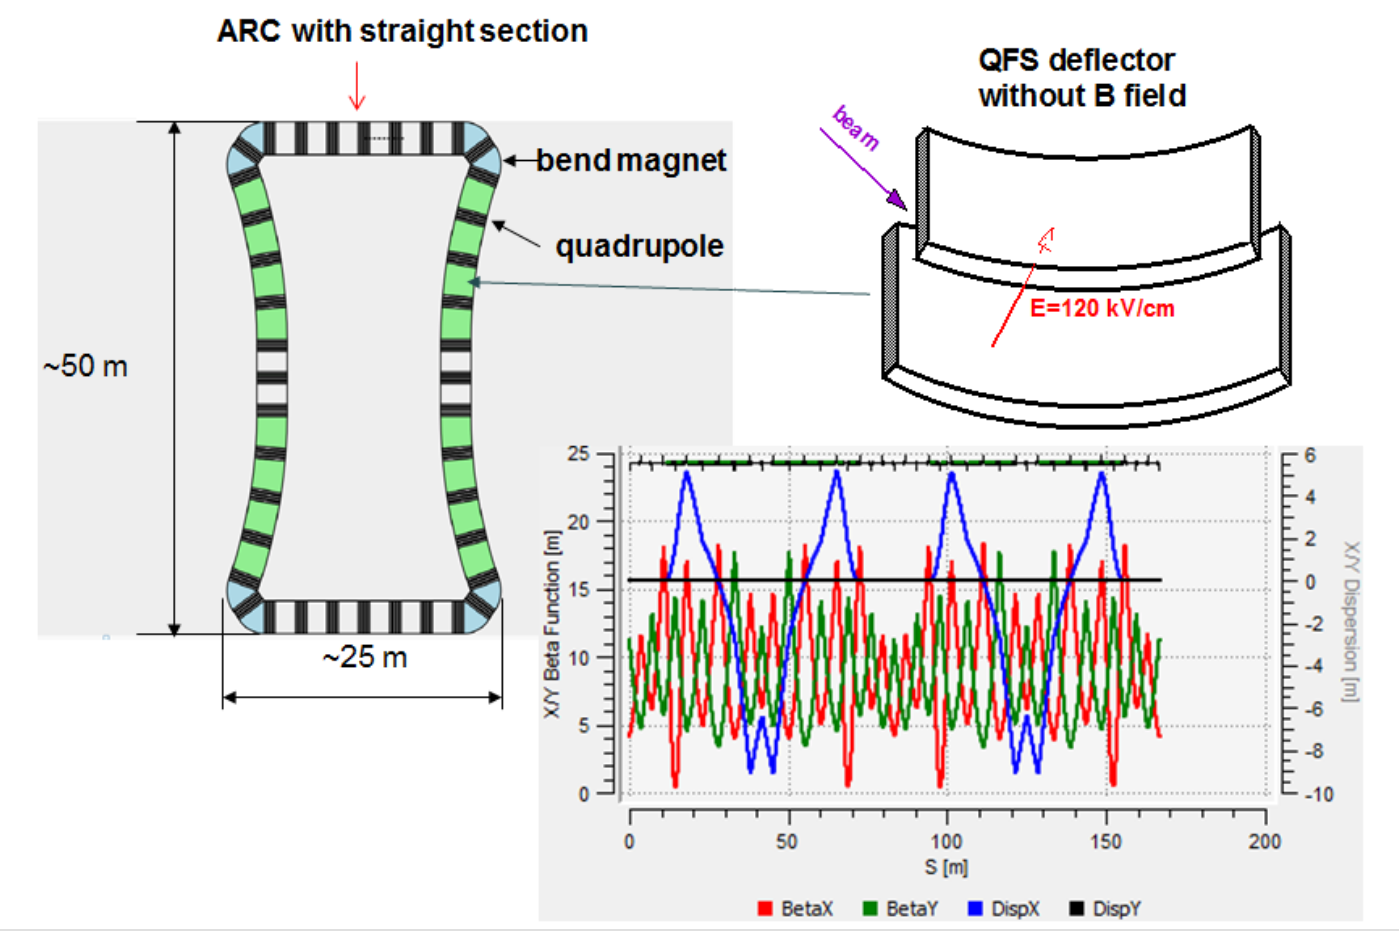
\includegraphics[width=\linewidth]{images/chapter2/6_3_lattice}
	\caption{Вариант кольца, построенного по принципу квази-замороженного спина, дизайн с разделением E- и B-полей. (Рисунок взят из~\cite{Senichev:Lattices})\label{fig:QFS_6_3_lattice}}
\end{figure}

\subsection{Структура с кодовым названием E+B}\label{chpt2:lattice:QFS:EB}

В структуре, представленной на Рисунке~\ref{fig:QFS_E+B_lattice}, используются прямые, статические фильтры Вина. Это позволяет:
\begin{enumerate*}[\itshape a\upshape)]
	\item исключить нелинейные компоненты электростатического поля, возникающие в связи с кривизной дефлектора, и 
	\item упростить структуру с инженерной точки зрения.
\end{enumerate*}

Длина структуры 149.21~м, энергия инжектируемых дейтронов 270 МэВ. Для подавления эффекта декогеренции первого порядка используется ВЧ-резонатор с продольным напряжением $V = 100$ кВ и частотой $f_{RF} = 5\cdot f_{rev}$, где $f_{rev} = 0.98$ МГц. Нелинейные эффекты декогеренции подавляются с помощью \hl{четырёх семейств секступолей}.
\begin{figure}[h!]
	\centering
	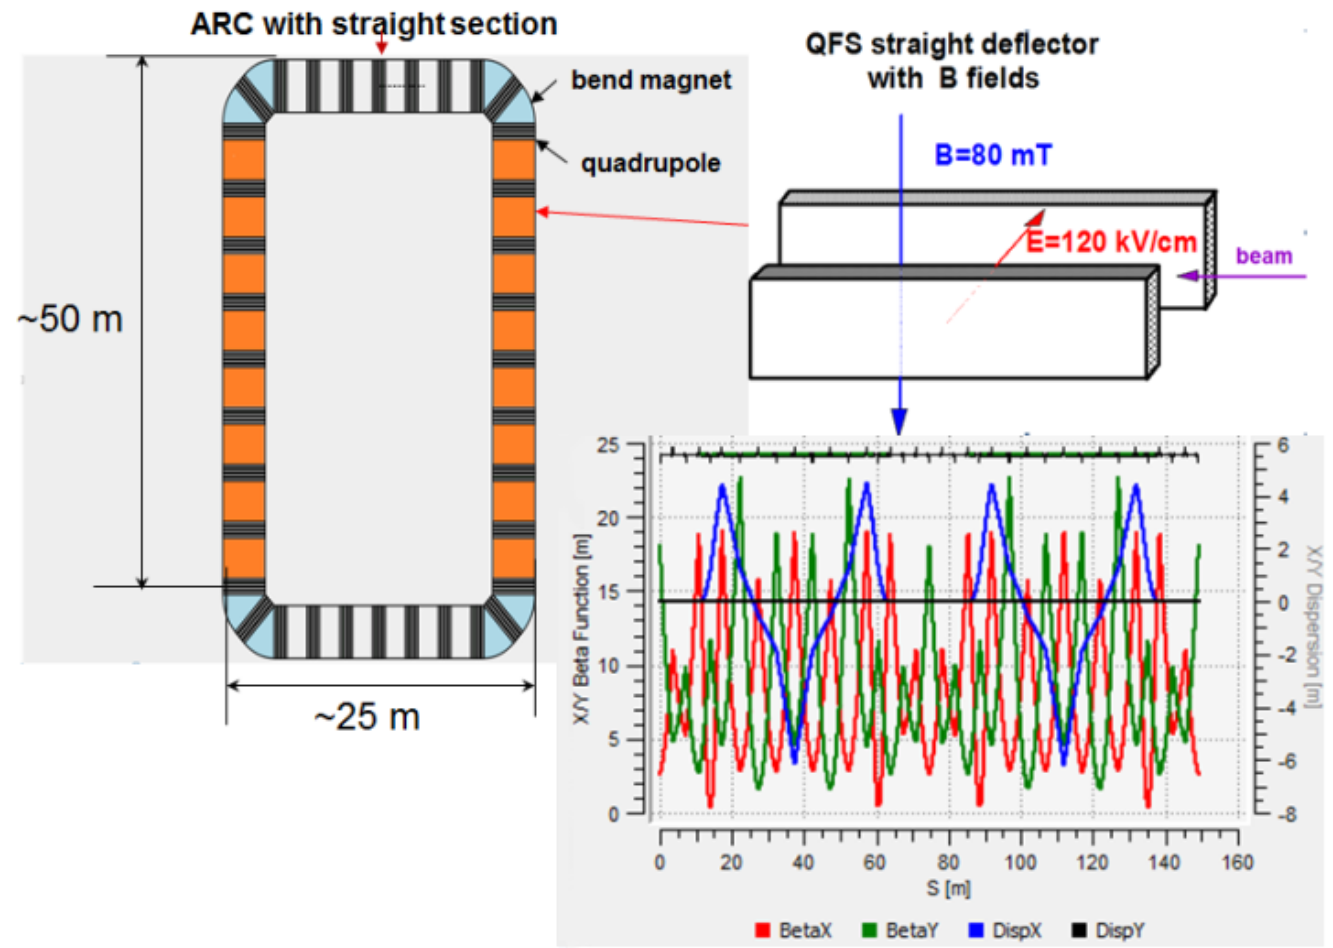
\includegraphics[width=\linewidth]{images/chapter2/E+B_lattice}
	\caption{Вариант кольца, построенного по принципу квази-замороженного спина, дизайн с прямыми фильтрами Вина. (Рисунок взят из~\cite{Senichev:Lattices})\label{fig:QFS_E+B_lattice}}
\end{figure}

